\chapter{Resultate}
\label{ch:resultate}

Die nächsten Absätze können gelöscht werden und sollen nur eine Einleitung in Latex bieten.

\section{Strukturierung}
\label{ch:resultate:strukturierung}

\begin{tabular}{ l p{5.256cm} l }
    Code                   & Beschreibung                                                                     & Level der Überschrift \\ \hline
    \verb|\capter{Text}| & legt ein Kapitel an                                                              & 1                     \\
    \verb|\capter*{Text}| & legt ein Kapitel an, das nicht im Inhaltsverzeichnis gelistet wird               & 1                     \\
    \verb|\section{Text}| & legt einen Abschnitte an                                                         & 2                     \\
    \verb|\subection{Text}| & legt einen Unterabschnitt an                                                     & 3                     \\
    \verb|\subsubsection{Text}| & legt einen Unterunterabschnit an, der nicht im Inhaltsverzeichnis angeführt wird & 4
\end{tabular}

\section{Referenzieren}

Man kann auch auf vorherige Abschnitt verweisen (siehe \autoref{ch:resultate:strukturierung}). Wenn man sich nur die Zahl des Abschnittes ohne das Wort Kapitel/Abschnitt/\dots ausgeben lassen möchte, verwendet man~\ref{ch:resultate:strukturierung}. Die Tilde verhindert, dass die Referenz auf eine neue Zeile umbricht.

\section{Zitieren}

In der Datei \verb|biblatex.bib| befindet sich die Information über die Quellen, auf die man verweisen möchte. Diese Datei kann man sich von einem ``reference management program'' z.B. Zotero\footnote{\href{https://www.zotero.org/}{https://www.zotero.org/}} generieren lassen. Wichtig ist, dass sie im Format Biblatex --- nicht Bibtex --- vorliegt. Jetzt kann auf diese Quelle auf mehrere Arten verweisen (die ersten zwei sind vermutlich am wichtigsten):

\begin{itemize}
    \item Wie auch \cite{appelman_rose_1998} herausgefunden haben, kann man die Namen verwenden.
    \item Gelegentlich wird aber nur in einer Klammer zitiert \parencite{appelman_rose_1998}.
    \item Vielleicht möchte man nur die Namen der Autoren \citeauthor[hier noch ein Zusatz]{appelman_rose_1998} anführen.
    \item Der Titel lautet \citetitle{appelman_rose_1998}
    \item Geschrieben wurde das Paper \citeyear{appelman_rose_1998}.
    \item \dots
\end{itemize}

\section{Abbildung}

Ganz leicht können Abbildungen eingefügt werden (siehe \autoref{fig:meine-abbildung}). Der Zusatz in eckigen Klammern setzt die Position der Grafik. Eine Beschreibung der möglichen Werte findet man auf dem entsprechenden Knowledgebase Eintrag\footnote{\href{https://www.overleaf.com/learn/latex/Positioning\_of\_Figures}{https://www.overleaf.com/learn/latex/Positioning\_of\_Figures}} von Overleaf.

Mit \verb|\includegraphics{dateiname-in-graphics-folder}| wird die eigentliche \newline Grafik eingefügt. Der Zusatz in eckigen Klammern legt die Größe fest. Die Anweisung \verb|width=0.75\textwidth| setzt die Breite der Grafik auf \sfrac{3}{4} des Seiteninhalts.

\begin{figure}[h]
    \centering
    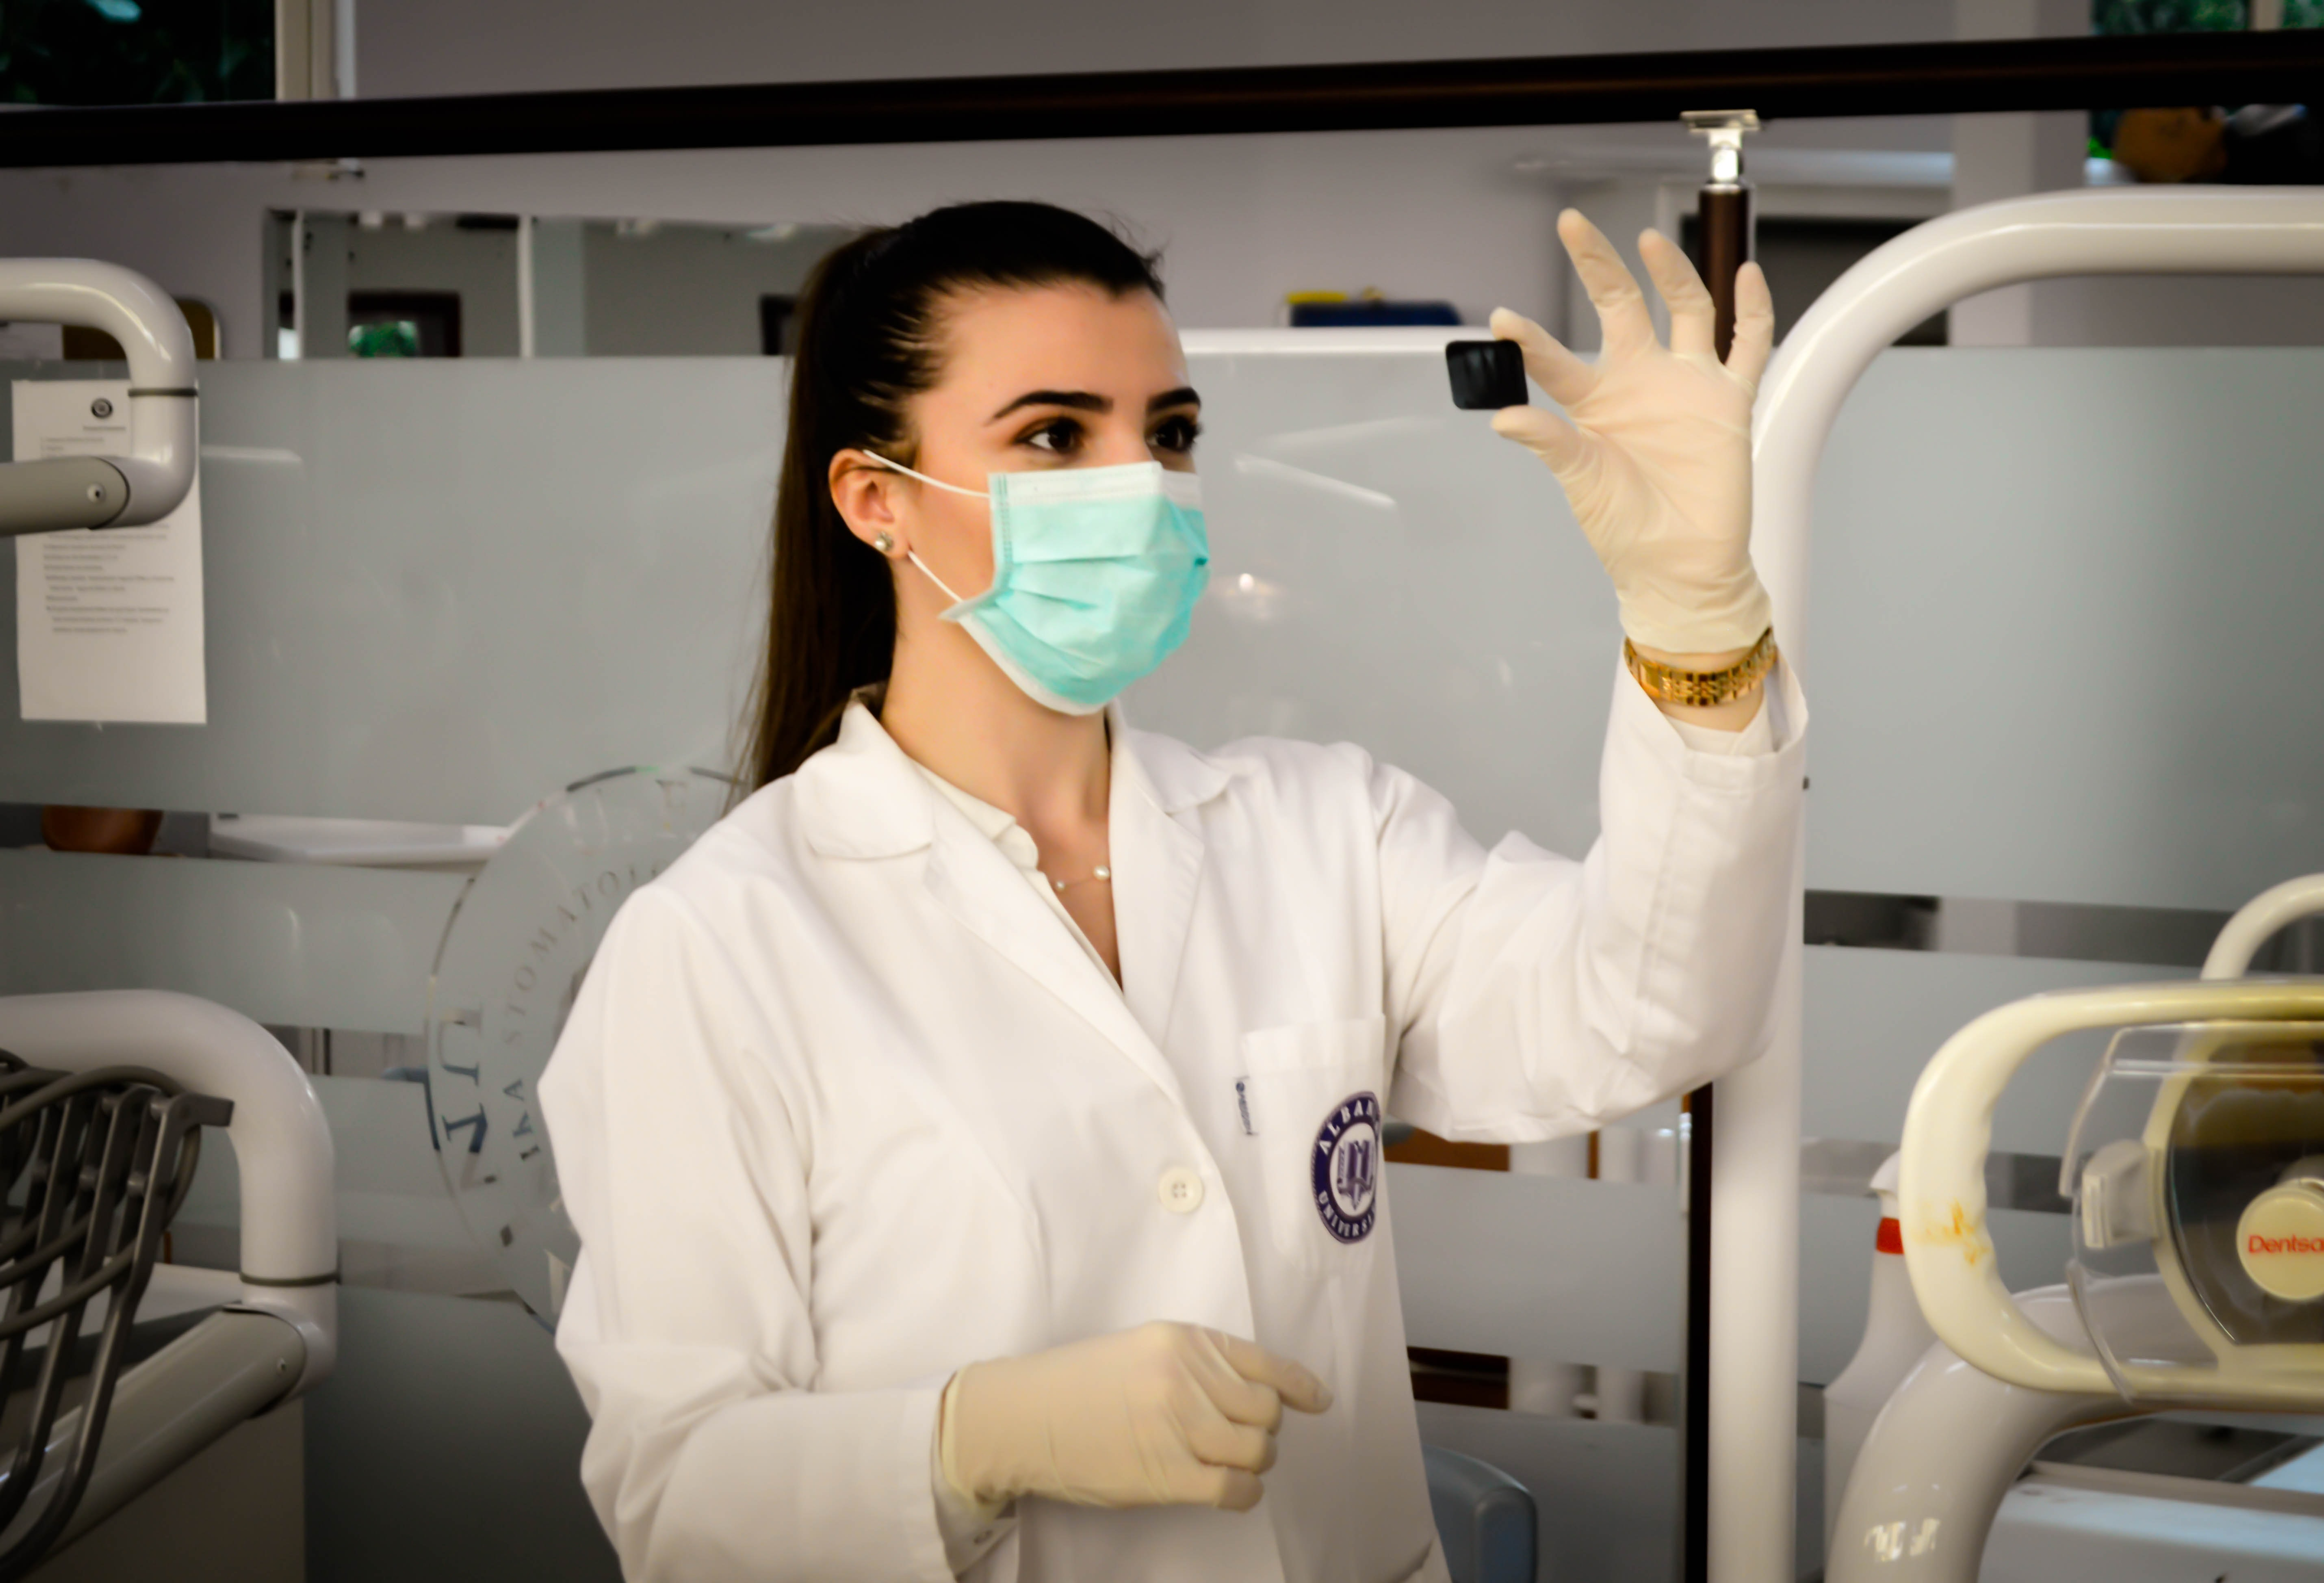
\includegraphics[width=0.75\textwidth]{ani-kolleshi.jpg}
    \caption{Meine erste Abbildung.}
    \label{fig:meine-abbildung}
\end{figure}

\newpage
\section{Tabellen}

Tabellen sind leider sehr unangenehm anzulegen. Die Website Tables Generator\footnote{\href{https://www.tablesgenerator.com/}{https://www.tablesgenerator.com/}} hilft allerdings. Ein Besipiel für eine simple Tabelle sieht man in \autoref{tab:meine-tabelle}.

\begin{table}[h]
    \centering
    \begin{tabular}{lll}
    \multicolumn{3}{l}{}                         \\
    id       & Vorname         & Nachname        \\ \hline
    1        & Max             & Mustermann      \\
    2        & Maximilia       & Musterfrau     
    \end{tabular}
    \caption{Meine erste Tabelle.}
    \label{tab:meine-tabelle}
\end{table}
